\documentclass[11pt]{article}

% ---------- Packages ----------
\usepackage[a4paper,margin=1in]{geometry}
\usepackage{booktabs}
\usepackage{tabularx}
\usepackage{longtable}
\usepackage{xcolor}
\usepackage[hidelinks]{hyperref}
\usepackage{tikz}
\usetikzlibrary{arrows.meta,positioning,shapes.multipart,fit,backgrounds,calc}
\usepackage{enumitem}
\usepackage{amsmath}
\usepackage{amssymb}
\usepackage{listings}
\usepackage{parskip}
\usepackage{titlesec}
\usepackage{fancyhdr}
\usepackage{array}
\usepackage{colortbl}
\usepackage{caption}
\usepackage{multicol}

% ---------- Colors ----------
\definecolor{navy}{RGB}{20,40,70}
\definecolor{steel}{RGB}{70,100,140}
\definecolor{lightgray}{RGB}{240,240,240}
\definecolor{accentgreen}{RGB}{40,110,70}
\definecolor{warnred}{RGB}{150,40,40}
\definecolor{codebg}{RGB}{245,245,245}

% ---------- Section styling ----------
\titleformat{\section}{\large\bfseries\color{navy}}{\thesection}{0.6em}{}
\titleformat{\subsection}{\normalsize\bfseries\color{steel}}{\thesubsection}{0.5em}{}
\titleformat{\subsubsection}{\normalsize\bfseries}{\thesubsubsection}{0.5em}{}

% ---------- Header/Footer ----------
\pagestyle{fancy}
\fancyhf{}
\fancyhead[L]{\small SIM-SM --- GPU Architecture \& Runtime Simulator}
\fancyhead[R]{\small Project Roadmap}
\fancyfoot[C]{\small\thepage}
\renewcommand{\headrulewidth}{0.4pt}

% ---------- Listings ----------
\lstset{
  basicstyle=\ttfamily\small,
  backgroundcolor=\color{codebg},
  frame=single,
  rulecolor=\color{lightgray},
  breaklines=true,
  columns=fullflexible,
  showstringspaces=false,
  xleftmargin=4pt,
  xrightmargin=4pt,
  aboveskip=8pt,
  belowskip=8pt
}

% ---------- Helper environments ----------
\newcommand{\statuslabel}[1]{\textbf{\textcolor{steel}{[#1]}}}
\newcommand{\guaranteed}{\textcolor{accentgreen}{\textbf{GUARANTEED}}}
\newcommand{\stretchtag}{\textcolor{warnred}{\textbf{STRETCH --- NOT REQUIRED FOR WEEK 1}}}
\newcommand{\postweek}{\textcolor{steel}{\textbf{POST-WEEK-1}}}

\hypersetup{
  pdftitle={SIM-SM Project Roadmap},
  pdfauthor={SIM-SM Project},
  colorlinks=true,
  linkcolor=steel,
  citecolor=steel,
  urlcolor=steel
}

\begin{document}

% =========================================================
% COVER PAGE
% =========================================================
\begin{titlepage}
\centering
\vspace*{2.5cm}

{\Huge \textbf{\textcolor{navy}{SIM-SM}}}

\vspace{0.5cm}
{\Large \textcolor{steel}{GPU Architecture \& Runtime Simulator}}

\vspace{1.5cm}

{\large Project Roadmap}\\[0.3cm]
{\normalsize Week 1 MVP + Post-Week-1 Extensions}

\vspace{1cm}

\begin{tabular}{c}
\textit{C++ / CMake / GoogleTest} \\
\textit{GPU Architecture / SIMT / Memory Systems / Scheduling}
\end{tabular}

\vspace{2cm}

\begin{minipage}{0.8\textwidth}
\centering
\small
SIM-SM is a deliberately scoped, CPU-based, educational GPU architecture and
runtime simulator written in C++. It models the conceptual GPU execution
hierarchy (GPU $\rightarrow$ SM $\rightarrow$ thread block $\rightarrow$ warp
$\rightarrow$ thread), a tiny SIMT instruction set, pluggable warp
scheduling policies, a multi-level cache and memory hierarchy, memory
coalescing, constrained divergence, block-level barrier synchronization, and
occupancy analysis. The project is built as a portfolio artifact for a
System Software Engineering internship application, and this document is
the authoritative roadmap covering the seven-day guaranteed MVP and every
planned extension beyond it.
\end{minipage}

\vspace{2cm}
{\small This document is a \textbf{roadmap}, not a status report. Items are
labeled \guaranteed{}, \stretchtag{}, or \postweek{} throughout --- nothing
described here should be read as already implemented unless explicitly
stated.}

\vfill
{\small Compiled with \texttt{pdflatex}. Source: \texttt{sim-sm-roadmap.tex}}
\end{titlepage}

\tableofcontents
\newpage

% =========================================================
% EXECUTIVE SUMMARY
% =========================================================
\section{Executive Summary}

SIM-SM is a CPU-based educational simulator of GPU architecture and
runtime behavior, written in C++. It exists to demonstrate --- concretely,
in working code --- an understanding of how a GPU organizes and executes
massively parallel work: the SM/block/warp/thread hierarchy, SIMT
instruction issue, warp scheduling policy, a multi-level memory and cache
hierarchy, memory coalescing, constrained control-flow divergence, barrier
synchronization, and occupancy.

The project is structured around a strict two-phase plan:

\begin{itemize}[leftmargin=1.2cm]
  \item \textbf{Week 1 (guaranteed MVP):} a seven-day, fully scoped build
  that produces a working simulator, one kernel (Vector Add), four
  mandatory controlled experiments, a real test suite, and a README with
  real measured results.
  \item \textbf{Post-Week-1 (extensions):} eight ordered extensions ---
  matrix multiply (if not finished in Week 1), a priority scheduler,
  additional cache replacement policies, a debug/trace mode, additional
  benchmark kernels, a transfer-cost model, a plotting pipeline, and
  optional \texttt{perf} profiling of the simulator itself.
\end{itemize}

Week 1 is intended to prove that a small, honestly-scoped systems project
can be built end-to-end, correctly, and measured --- not merely
prototyped. What Week 1 intentionally excludes (a second kernel, general
divergence/reconvergence, additional scheduler and cache policies, tracing,
transfer modeling, visualization, and any self-profiling) is exactly the
material the post-Week-1 roadmap picks up, always building on interfaces
that Week 1 already stabilizes (\texttt{WarpScheduler},
\texttt{ReplacementPolicy}, the \texttt{PerformanceCounter} event taps, and
the kernel-launch plumbing) rather than requiring rework.

\begin{center}
\fbox{\begin{minipage}{0.85\textwidth}
\centering
\textbf{The project is intentionally small but genuinely working, rather
than broad and half-finished.}
\end{minipage}}
\end{center}

% =========================================================
% NVIDIA APPLICATION POSITIONING
% =========================================================
\section{Relevance to a System Software Engineering Role}

SIM-SM is built as a portfolio project for a System Software Engineering
internship application. Its relevance rests on a specific, honest
technical story, not on any claim of building real GPU software:

\begin{center}
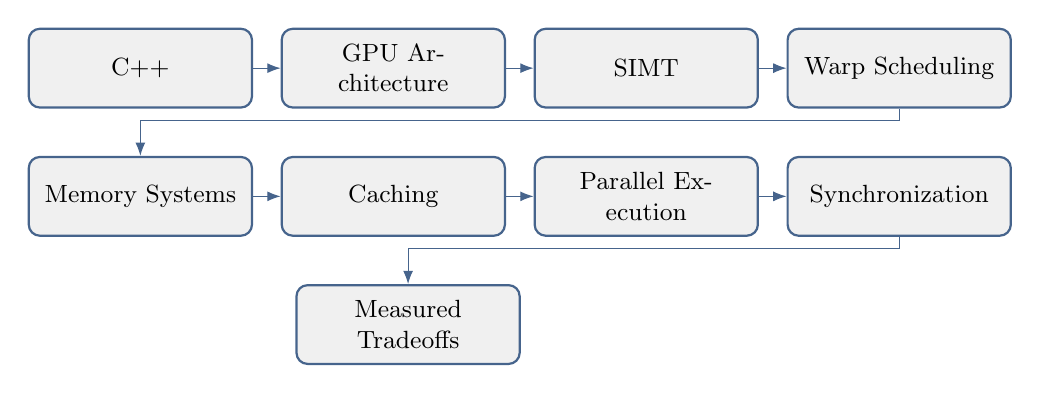
\begin{tikzpicture}[
  node distance=0.35cm and 0.35cm,
  every node/.style={font=\small},
  box/.style={draw=steel, thick, rounded corners, fill=lightgray,
    text width=2.6cm, align=center, minimum height=1cm}
]
\node[box] (a) {C++};
\node[box, right=of a] (b) {GPU Architecture};
\node[box, right=of b] (c) {SIMT};
\node[box, right=of c] (d) {Warp Scheduling};
\node[box, below=0.6cm of a] (e) {Memory Systems};
\node[box, right=of e] (f) {Caching};
\node[box, right=of f] (g) {Parallel Execution};
\node[box, right=of g] (h) {Synchronization};
\node[box, below=0.6cm of e, xshift=3.4cm] (i) {Measured Tradeoffs};

\draw[-{Latex}, steel] (a) -- (b);
\draw[-{Latex}, steel] (b) -- (c);
\draw[-{Latex}, steel] (c) -- (d);
\draw[-{Latex}, steel] (d.south) -- ++(0,-0.15) -| (e.north);
\draw[-{Latex}, steel] (e) -- (f);
\draw[-{Latex}, steel] (f) -- (g);
\draw[-{Latex}, steel] (g) -- (h);
\draw[-{Latex}, steel] (h.south) -- ++(0,-0.15) -| (i.north);
\end{tikzpicture}
\end{center}

This project demonstrates systems-level reasoning about hardware/software
execution models: how work is decomposed and scheduled, how a memory
hierarchy is organized and why cache behavior matters, how synchronization
correctness is enforced, and how architectural choices are evaluated with
real measurements rather than intuition.

\subsection{Explicit Non-Claims}

To avoid any ambiguity, SIM-SM does \textbf{not} claim, and is not
intended to demonstrate, any of the following:

\begin{multicols}{2}
\begin{itemize}[leftmargin=1cm]
  \item CUDA implementation
  \item CUDA runtime development
  \item HIP development
  \item OpenGL development
  \item DirectX development
  \item GPU driver development
  \item OS kernel development
  \item Microcode development
  \item PTX compatibility
  \item NVIDIA hardware fidelity
  \item Real NVIDIA performance characteristics
\end{itemize}
\end{multicols}

\subsection{Simulated Metrics vs. Host Execution}
\label{sec:sim-vs-host}

A recurring distinction runs through the entire project and this document:

\begin{center}
\begin{tabularx}{\textwidth}{@{}l X@{}}
\toprule
\textbf{Category} & \textbf{What it actually measures} \\
\midrule
Simulated GPU metrics (cycles, IPC, stalls, cache hits/misses, memory
transactions, occupancy) & Properties of the \emph{simulated} GPU model,
computed by simulator logic. These are not measurements of the host CPU
running the simulator. \\
\addlinespace
Host process measurements (e.g. Linux \texttt{perf} output, if used in
Extension~7) & Properties of the \emph{actual C++ process} executing the
simulator on the host CPU --- wall-clock time, host cache misses,
instructions retired by the host. \\
\bottomrule
\end{tabularx}
\end{center}

These two categories are never conflated anywhere in this document, in the
simulator's output, or in the project README.

% =========================================================
% PROJECT GOALS
% =========================================================
\section{Project Goals}

\begin{longtable}{@{}p{4cm}p{10.5cm}@{}}
\toprule
\textbf{Goal} & \textbf{Description} \\
\midrule
\endhead
GPU hierarchy & Model the GPU $\rightarrow$ SM $\rightarrow$ thread block
$\rightarrow$ warp $\rightarrow$ thread decomposition of a kernel launch. \\
SIMT execution & Execute a tiny instruction set across a warp of threads in
lockstep, in the SIMT style. \\
Warp scheduling & Implement and compare pluggable scheduling policies
(Round-Robin, Greedy) that select which resident warp issues each cycle. \\
Memory hierarchy & Model registers, shared memory, global memory, and a
multi-level cache (L1 per-SM, shared L2). \\
Cache behavior & Implement a configurable set/line/associativity cache with
LRU replacement and measurable hit/miss/eviction behavior. \\
Coalescing & Classify a warp's memory addresses into transactions and show
the measured effect of contiguous vs.\ strided access patterns. \\
Synchronization & Implement block-level barrier synchronization, including
detection of malformed/divergent barrier usage so the simulator cannot
silently hang. \\
Occupancy & Compute occupancy from resource inputs (registers/thread,
shared memory/block, threads/block, SM limits) and resulting resident
blocks/active warps. \\
Benchmarking & Run controlled experiments that isolate one architectural
variable at a time and report real measured results. \\
Testing & Validate every component (hierarchy, execution, scheduling,
cache, memory, synchronization, occupancy) with a meaningful GoogleTest
suite. \\
\bottomrule
\end{longtable}

% =========================================================
% SCOPE BOUNDARIES
% =========================================================
\section{Scope Boundaries}

\begin{longtable}{@{}p{7cm}p{7.5cm}@{}}
\toprule
\textbf{In Scope} & \textbf{Explicitly Out of Scope} \\
\midrule
\endhead
GPU/SM/block/warp/thread hierarchy & Real CUDA/PTX compatibility \\
Tiny custom ISA (ADD, SUB, MUL, LOAD, STORE, MOV, CMP, BRANCH, BARRIER) &
NVIDIA hardware fidelity of any kind \\
Round-Robin and Greedy warp scheduling & Full production-grade GPU
modeling \\
Performance counters (cycles, IPC, stalls) & CUDA runtime, HIP, OpenGL, or
DirectX development \\
Register file, shared memory, global memory & GPU driver or OS kernel
development \\
Set/line/associativity cache with LRU, per-SM L1, shared L2, AMAT &
Microcode development \\
Memory coalescing (contiguous vs.\ strided) & General-purpose
divergence/reconvergence stack (Week 1 only supports one constrained
branch pattern) \\
Constrained SIMT divergence (single branch pattern) & Phase~2
functionality being pulled forward into Week 1 \\
Block-level barrier synchronization with malformed-barrier detection &
Tiled Matrix Multiply as a Week~1 requirement (it is stretch-only) \\
Occupancy calculation & Fabricated or placeholder benchmark numbers \\
Vector Add kernel (guaranteed) & Claiming any real NVIDIA performance
characteristics \\
Four mandatory controlled experiments & Unnecessary architectural
sophistication for its own sake \\
GoogleTest suite and CSV-based measured results & \\
\bottomrule
\end{longtable}

% =========================================================
% HIGH-LEVEL ARCHITECTURE
% =========================================================
\section{High-Level Architecture}

\subsection{Structural Hierarchy}

\begin{center}
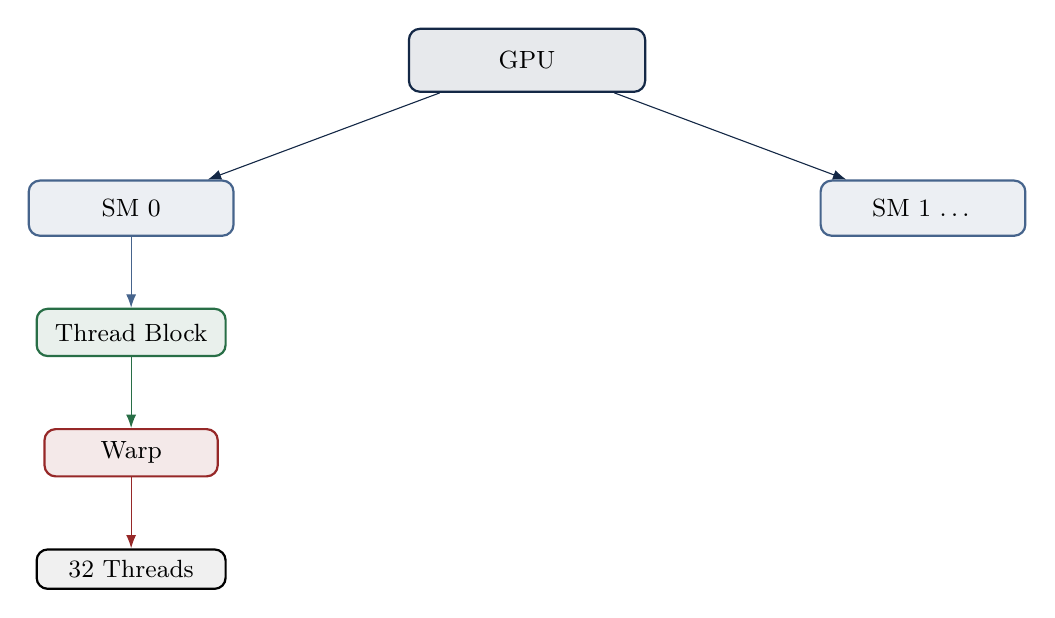
\begin{tikzpicture}[
  every node/.style={font=\small},
  gpu/.style={draw=navy, thick, fill=navy!10, rounded corners, minimum width=3cm, minimum height=0.8cm, align=center},
  sm/.style={draw=steel, thick, fill=steel!10, rounded corners, minimum width=2.6cm, minimum height=0.7cm, align=center},
  blk/.style={draw=accentgreen, thick, fill=accentgreen!10, rounded corners, minimum width=2.4cm, minimum height=0.6cm, align=center},
  warp/.style={draw=warnred, thick, fill=warnred!10, rounded corners, minimum width=2.2cm, minimum height=0.6cm, align=center},
  thr/.style={draw=black, thick, fill=lightgray, rounded corners, minimum width=2.4cm, minimum height=0.5cm, align=center},
  level distance=1.3cm
]
\node[gpu] (gpu) {GPU};
\node[sm, below left=1.1cm and 2.2cm of gpu] (sm0) {SM 0};
\node[sm, below right=1.1cm and 2.2cm of gpu] (sm1) {SM 1 \ldots};
\node[blk, below=0.9cm of sm0] (blk0) {Thread Block};
\node[warp, below=0.9cm of blk0] (warp0) {Warp};
\node[thr, below=0.9cm of warp0] (thr0) {32 Threads};

\draw[-{Latex}, navy] (gpu) -- (sm0);
\draw[-{Latex}, navy] (gpu) -- (sm1);
\draw[-{Latex}, steel] (sm0) -- (blk0);
\draw[-{Latex}, accentgreen] (blk0) -- (warp0);
\draw[-{Latex}, warnred] (warp0) -- (thr0);
\end{tikzpicture}
\end{center}

Each SM holds one or more resident thread blocks (subject to occupancy
limits); each thread block decomposes into warps of 32 threads; each warp
executes the tiny SIMT instruction set in lockstep.

\subsection{Conceptual Execution Flow}

\begin{center}
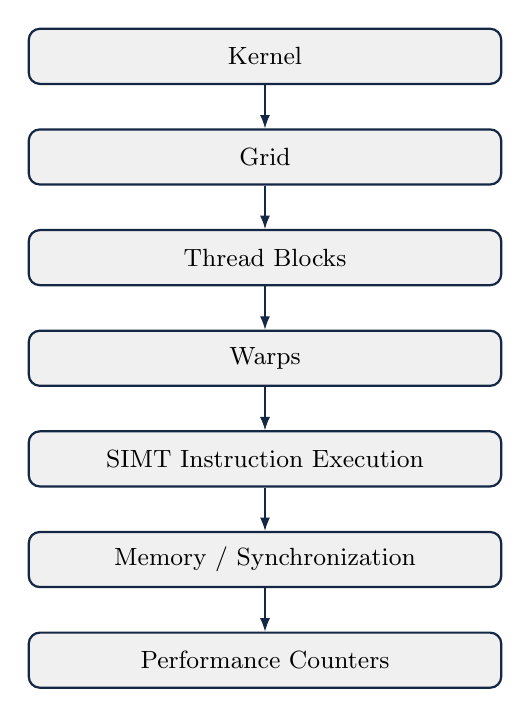
\begin{tikzpicture}[
  every node/.style={font=\small},
  stage/.style={draw=navy, thick, fill=lightgray, rounded corners, minimum width=6cm, minimum height=0.7cm, align=center},
  node distance=0.55cm
]
\node[stage] (k) {Kernel};
\node[stage, below=of k] (g) {Grid};
\node[stage, below=of g] (tb) {Thread Blocks};
\node[stage, below=of tb] (w) {Warps};
\node[stage, below=of w] (simt) {SIMT Instruction Execution};
\node[stage, below=of simt] (mem) {Memory / Synchronization};
\node[stage, below=of mem] (perf) {Performance Counters};

\foreach \a/\b in {k/g, g/tb, tb/w, w/simt, simt/mem, mem/perf}
  \draw[-{Latex}, navy] (\a) -- (\b);
\end{tikzpicture}
\end{center}

\subsection{Execution Model (Detailed)}

The diagram below expands the last three stages above --- SIMT
instruction execution, memory, and synchronization --- into the concrete
components that implement them, so the whole pipeline from kernel launch
to memory access is visible in one picture.

\begin{center}
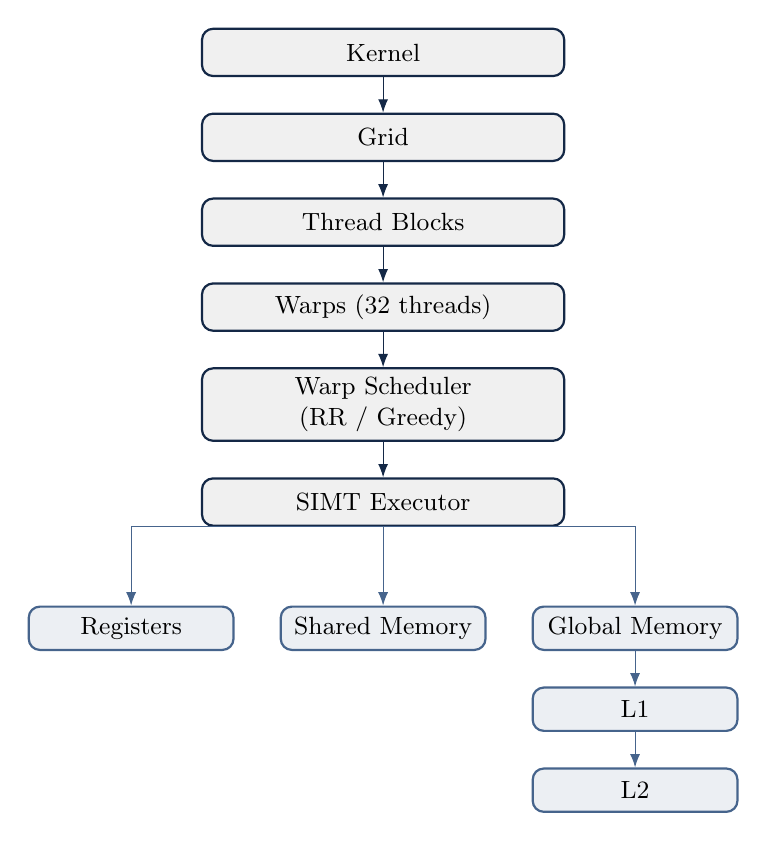
\begin{tikzpicture}[
  every node/.style={font=\small},
  stage/.style={draw=navy, thick, fill=lightgray, rounded corners, minimum width=4.6cm, minimum height=0.6cm, align=center},
  memnode/.style={draw=steel, thick, fill=steel!10, rounded corners, minimum width=2.6cm, minimum height=0.55cm, align=center},
  node distance=0.45cm
]
\node[stage] (k) {Kernel};
\node[stage, below=of k] (g) {Grid};
\node[stage, below=of g] (tb) {Thread Blocks};
\node[stage, below=of tb] (w) {Warps (32 threads)};
\node[stage, below=of w] (sched) {Warp Scheduler\\(RR / Greedy)};
\node[stage, below=of sched] (simt) {SIMT Executor};

\node[memnode, below=1.0cm of simt, xshift=-3.2cm] (reg) {Registers};
\node[memnode, below=1.0cm of simt] (shm) {Shared Memory};
\node[memnode, below=1.0cm of simt, xshift=3.2cm] (gm) {Global Memory};
\node[memnode, below=of gm] (l1) {L1};
\node[memnode, below=of l1] (l2) {L2};

\foreach \a/\b in {k/g, g/tb, tb/w, w/sched, sched/simt}
  \draw[-{Latex}, navy] (\a) -- (\b);
\draw[-{Latex}, steel] (simt.south) -| (reg.north);
\draw[-{Latex}, steel] (simt.south) -- (shm.north);
\draw[-{Latex}, steel] (simt.south) -| (gm.north);
\draw[-{Latex}, steel] (gm) -- (l1);
\draw[-{Latex}, steel] (l1) -- (l2);
\end{tikzpicture}
\end{center}

As detailed in Section~\ref{sec:day4}, registers and shared memory are direct,
non-cached accesses from the SIMT executor, while global-memory accesses
are the only ones that traverse the L1/L2 cache path.

% =========================================================
% CORE HIERARCHY
% =========================================================
\section{Core Hierarchy}

\begin{description}[leftmargin=1.2cm, style=nextline]
  \item[GPU] The top-level simulated device, owning a fixed number of SMs.
  \item[SM (Streaming Multiprocessor)] A simulated execution unit that
  holds resident thread blocks and issues warp instructions each cycle
  according to the active scheduling policy.
  \item[Grid] The full set of thread blocks launched by a kernel.
  \item[Thread Block] A group of threads that share shared memory and can
  synchronize via a block-level barrier.
  \item[Warp] A group of 32 threads executed together in lockstep (SIMT).
  \item[Thread] The smallest unit of simulated execution, holding its own
  registers and program counter state within a warp.
  \item[Kernel] The unit of work launched onto the grid --- in Week~1,
  Vector Add.
\end{description}

This representation is deliberately simplified relative to real hardware
--- it exists to make the architectural concepts (decomposition,
scheduling, memory hierarchy, synchronization) inspectable and testable,
not to reproduce real SM microarchitecture.

The warp size is fixed:
\[
\text{Warp Size} = 32
\]
This reflects the familiar NVIDIA warp abstraction as a modeling choice
made for pedagogical clarity, not a claim that SIM-SM reproduces real
hardware internals.

% =========================================================
% WEEK 1 MVP
% =========================================================
\section{Week 1 MVP}

\begin{center}
\fbox{\begin{minipage}{0.85\textwidth}
\centering
\textbf{Week 1 is the guaranteed MVP.}
\end{minipage}}
\end{center}

The complete guaranteed Week~1 deliverable, all items \guaranteed{}:

\begin{enumerate}[leftmargin=1.2cm]
  \item C++ / CMake project
  \item GoogleTest test suite
  \item JSON configuration (\texttt{nlohmann/json})
  \item GPU $\rightarrow$ SM $\rightarrow$ Block $\rightarrow$ Warp
  $\rightarrow$ Thread hierarchy
  \item Tiny toy instruction set and instruction execution
  \item Round-Robin warp scheduler
  \item Greedy warp scheduler
  \item Performance counters: cycles, instructions retired, IPC, stall
  reasons
  \item Register file
  \item Shared memory
  \item Global memory
  \item Set/line/associativity-based cache
  \item LRU replacement
  \item Per-SM L1 cache
  \item Shared L2 cache
  \item AMAT calculation
  \item Memory coalescing
  \item Basic constrained SIMT divergence (single supported branch
  pattern)
  \item Block-level barrier synchronization (with malformed-barrier
  detection)
  \item Occupancy calculation
  \item Vector Add kernel
  \item Four controlled experiments
  \item CSV output with real measured results
  \item Meaningful GoogleTests
  \item README with architecture/design/limitations/actual results
\end{enumerate}

\begin{center}
\fbox{\begin{minipage}{0.85\textwidth}
\textbf{All 25 deliverables are mandatory.} The only permitted reduction
is within the implementation complexity of constrained divergence: if
time is limited, Week~1 falls back to the single supported branch pattern
rather than attempting sophisticated reconvergence. The sacrifice order in
Section~\ref{sec:sacrifice} governs what is cut \emph{before} any of these
twenty-five items, never the items themselves.
\end{minipage}}
\end{center}

% =========================================================
% WEEK 1 DAY-BY-DAY ROADMAP
% =========================================================
\section{Week 1 Day-by-Day Roadmap}

\subsection{Day 1 --- Skeleton + Thread Hierarchy}
\statuslabel{Planned for Week 1} --- feasibility: 90--100\%

\textbf{Build:}
\begin{itemize}[leftmargin=1.2cm]
  \item Repository structure and CMake project
  \item GoogleTest integration via \texttt{FetchContent}
  \item \texttt{nlohmann/json} configuration loading
  \item \texttt{GPU}, \texttt{SM}, \texttt{Grid}, \texttt{ThreadBlock},
  \texttt{Warp}, \texttt{Thread}, \texttt{Kernel} classes (construction
  only at this stage)
  \item CLI entry point
\end{itemize}

\textbf{Proof of done:}
\begin{lstlisting}
$ ./gpu-sim --config configs/small_gpu.json --threads 1024
Grid: 1024 threads -> 32 warps -> 8 blocks -> scheduled across 4 SMs
\end{lstlisting}

\textbf{Required hierarchy edge cases (tested):}
\begin{itemize}[leftmargin=1.2cm]
  \item Non-multiple-of-32 thread counts
  \item Non-multiple-of-block-size counts
  \item Empty grid
\end{itemize}

\subsection{Day 2 --- Instruction Execution}
\statuslabel{Planned for Week 1} --- feasibility: 90\%

\textbf{Build:}
\begin{itemize}[leftmargin=1.2cm]
  \item \texttt{Instruction} and \texttt{Opcode}: \texttt{ADD}, \texttt{SUB},
  \texttt{MUL}, \texttt{LOAD}, \texttt{STORE}, \texttt{MOV}, \texttt{CMP},
  \texttt{BRANCH}, \texttt{BARRIER}
  \item \texttt{InstructionExecutor} for a single warp, straight-line
  execution
  \item Register state and memory state tracking
\end{itemize}

The ISA is intentionally tiny --- this is what keeps Week~1 feasible in
seven days; extra instructions beyond this minimum are explicitly the
lowest-priority sacrifice item (Section~\ref{sec:sacrifice}).

\textbf{Proof of done:} a hardcoded 5-instruction kernel runs to
completion; register and memory state are checked against hand-computed
values in a unit test.

\subsection{Day 3 --- Warp Scheduling}
\statuslabel{Planned for Week 1} --- feasibility: 85--95\%

\begin{center}
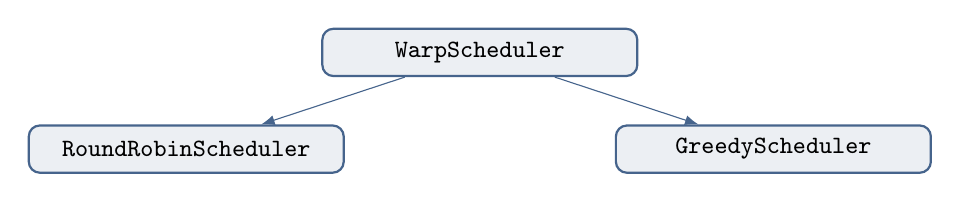
\begin{tikzpicture}[
  every node/.style={font=\small\ttfamily},
  box/.style={draw=steel, thick, rounded corners, fill=steel!10, minimum width=4cm, minimum height=0.6cm}
]
\node[box] (ws) {WarpScheduler};
\node[box, below left=0.6cm and -0.3cm of ws] (rr) {RoundRobinScheduler};
\node[box, below right=0.6cm and -0.3cm of ws] (gr) {GreedyScheduler};
\draw[-{Latex}, steel] (ws) -- (rr);
\draw[-{Latex}, steel] (ws) -- (gr);
\end{tikzpicture}
\end{center}

\textbf{Build:}
\begin{itemize}[leftmargin=1.2cm]
  \item \texttt{WarpScheduler} interface with a ready-warp selection
  contract
  \item SM holds multiple resident warps; one warp is issued/selected per
  cycle via the active policy
  \item \texttt{PerformanceCounter}: cycles, instructions retired, IPC,
  per-warp stall reasons
\end{itemize}

Round-Robin vs.\ Greedy is the project's most important architectural
experiment: it isolates scheduling policy as the sole variable and shows a
measurable, explainable difference in cycle count and IPC. No benchmark
numbers are invented here --- Section~\ref{sec:measurement-integrity}
governs measurement integrity for this and every experiment.

\textbf{Proof of done:}
\begin{lstlisting}
$ ./gpu-sim --config configs/small_gpu.json --kernel dummy --scheduler roundrobin
$ ./gpu-sim --config configs/small_gpu.json --kernel dummy --scheduler greedy
\end{lstlisting}
CSV rows differ between the two runs, and the difference is explainable
from the scheduling policy.

\subsection{Day 4 --- Memory Hierarchy}
\label{sec:day4}
\statuslabel{Planned for Week 1} --- feasibility: 80--90\%

\begin{center}
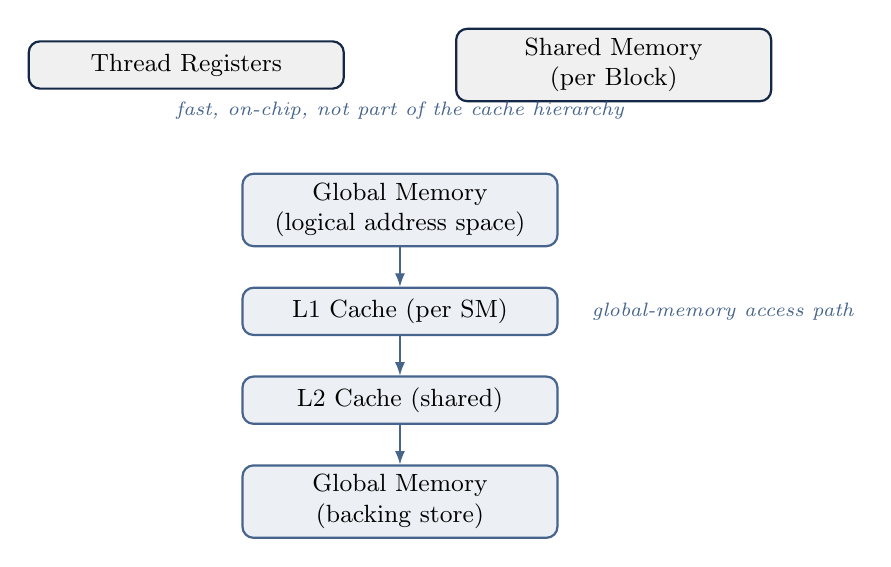
\begin{tikzpicture}[
  every node/.style={font=\small},
  stage/.style={draw=navy, thick, fill=lightgray, rounded corners, minimum width=4cm, minimum height=0.6cm, align=center},
  pathbox/.style={draw=steel, thick, fill=steel!10, rounded corners, minimum width=4cm, minimum height=0.6cm, align=center},
  lbl/.style={font=\scriptsize\itshape, text=steel},
  node distance=0.5cm
]
\node[stage] (reg) {Thread Registers};
\node[stage, right=1.4cm of reg] (shm) {Shared Memory\\(per Block)};
\node[lbl, below=0.35cm of $(reg)!0.5!(shm)$] (fastlbl) {fast, on-chip, not part of the cache hierarchy};

\node[pathbox, below=0.55cm of fastlbl] (gm1) {Global Memory\\(logical address space)};
\node[pathbox, below=of gm1] (l1) {L1 Cache (per SM)};
\node[pathbox, below=of l1] (l2) {L2 Cache (shared)};
\node[pathbox, below=of l2] (gm2) {Global Memory\\(backing store)};
\node[lbl, right=0.3cm of l1] {global-memory access path};

\draw[-{Latex}, steel] (gm1) -- (l1);
\draw[-{Latex}, steel] (l1) -- (l2);
\draw[-{Latex}, steel] (l2) -- (gm2);
\end{tikzpicture}
\end{center}

Thread registers and per-block shared memory are modeled as fast,
programmer-managed storage tiers --- they are \textbf{not} additional
levels of the cache hierarchy. Only accesses to the logical global-memory
address space traverse the simulated L1/L2 cache path before reaching
global memory's backing store. Keeping these paths visually and
conceptually separate matters: collapsing shared memory into the same
chain as L1/L2 would misleadingly suggest it is cached and evictable the
way global-memory data is, when in the simulator (as on real hardware) it
is explicitly allocated, block-scoped storage with no replacement policy
of its own.

\textbf{Build:}
\begin{itemize}[leftmargin=1.2cm]
  \item \texttt{RegisterFile}, \texttt{SharedMemory}, \texttt{GlobalMemory}
  \item \texttt{Cache} with configurable sets, line size, associativity
  \item A \texttt{ReplacementPolicy} interface with \texttt{LRUPolicy} as
  its sole Week~1 implementation --- LRU is the only replacement behavior
  Week~1 requires, but it is deliberately implemented behind this small
  interface (rather than hardcoded into \texttt{Cache}) so that
  Extension~2's \texttt{FIFOPolicy} and \texttt{RandomPolicy} can be added
  later without modifying cache logic. This is a small, low-cost
  abstraction with a clear, already-planned Phase~2 payoff --- not
  speculative overengineering.
  \item Cache statistics tracking
  \item Per-SM L1 cache and shared L2 cache
  \item AMAT (Average Memory Access Time) computation
\end{itemize}

The cache logic itself is not the primary risk; integrating it correctly
with the execution loop is where time actually goes, and Day~4 is budgeted
accordingly rather than assumed to be trivially easy.

\textbf{Proof of done:} unit tests hand-trace a small fixed access sequence

through a tiny cache configuration and assert exact hit/miss/eviction
outcomes.

\subsection{Day 5 --- GPU-Specific Execution Behavior}
\statuslabel{Planned for Week 1} --- feasibility: 60--80\% (the danger day)

\textbf{Memory Coalescing:}
\begin{itemize}[leftmargin=1.2cm]
  \item Classify a warp's addresses into transactions
  \item Compare contiguous access (\texttt{thread\_i -> base+i}) vs.\
  strided access (\texttt{thread\_i -> base+i*stride})
\end{itemize}

\textbf{Basic SIMT Divergence:}
\begin{center}
\fbox{\begin{minipage}{0.85\textwidth}
\centering
\textbf{Do not build a general-purpose reconvergence stack.}
\end{minipage}}
\end{center}
Support only the constrained divergence pattern needed for Week~1, using
the example \texttt{if (thread\_id \% 2 == 0)}.

\textbf{Barrier Synchronization:}
\begin{itemize}[leftmargin=1.2cm]
  \item Block-level barrier: threads stall until all required participants
  arrive
  \item Divergent barrier detection: a case where only some threads in a
  branch reach the barrier must be \textbf{detected and reported}, not
  silently hung
  \item This is a correctness requirement, not a nice-to-have --- an
  unhandled case here means the simulator can hang during its own demo
\end{itemize}

\textbf{Escape hatch:} if this day runs long, divergence complexity is cut
immediately --- drop to the single supported branch pattern and move on;
divergence debugging must not eat into Day~6.

\textbf{Proof of done:} the coalescing experiment shows fewer transactions
for contiguous access than for strided access (illustrative example from
planning: contiguous $\to$ 32 transactions, strided $\to$ 1024
transactions --- actual numbers come only from real runs). The divergence
benchmark shows more cycles for the divergent case than the uniform case.

\subsection{Day 6 --- Benchmarking + Occupancy}
\statuslabel{Planned for Week 1} --- feasibility: 70--90\% if Days 1--5
went well

\textbf{Vector Add (guaranteed kernel):} Vector Add is the guaranteed
Week~1 kernel. It is sufficient on its own because the four controlled
experiments --- not kernel count --- are the actual interview artifact; a
second kernel adds less signal than a fifth experiment would, and matrix
multiply's shared-memory tiling is real implementation risk this late in
the week.

\textbf{Occupancy:} computed from registers/thread, shared memory/block,
threads/block, and SM limits, producing resident blocks, active warps, and
occupancy.

\textbf{Four Required Experiments (all mandatory, none optional):}

\begin{center}
\begin{tabularx}{\textwidth}{@{}p{3.6cm}p{3.6cm}X@{}}
\toprule
\textbf{Experiment} & \textbf{Variables} & \textbf{Metrics} \\
\midrule
RR vs.\ Greedy & scheduler & cycles, IPC, stalls \\
Small vs.\ Large L1 & cache size & hit rate, AMAT \\
Coalesced vs.\ Strided & access pattern & memory transactions, effective
bandwidth \\
Small vs.\ Large Block & block size & occupancy, throughput \\
\bottomrule
\end{tabularx}
\end{center}

\begin{center}
\fbox{\begin{minipage}{0.85\textwidth}
\centering
All four experiments are mandatory and protected from the sacrifice
order.
\end{minipage}}
\end{center}

\textbf{Stretch (only if Days 1--5 finished on schedule):} Tiled Matrix
Multiply --- the first thing to drop if behind schedule. Vector Add alone,
run through all four experiments, is already a complete and defensible
artifact (see Section~\ref{sec:matmul-stretch}).

\textbf{Proof of done:} \texttt{/results/*.csv} populated with real numbers
from real runs for all four experiments; kernel count is one or two
depending on how the week went, and either is a valid submission.

\subsection{Day 7 --- Hardening + Documentation}
\label{sec:day7}
\statuslabel{Planned for Week 1} --- feasibility: 100\% only if no new
features are added

\textbf{Do:}
\begin{itemize}[leftmargin=1.2cm]
  \item GoogleTest cleanup and edge-case coverage --- target
  approximately 30--50 meaningful tests covering cache eviction, warp
  formation, thread indexing, scheduler selection, memory access, barrier
  behavior, and instruction execution. This target is a plan, not a
  guaranteed final count: the actual number reported in the README must be
  the real, measured test count from the final \texttt{ctest} run, whatever
  it turns out to be.
  \item README: motivation, architecture diagram, design decisions,
  execution model, memory hierarchy, scheduler, synchronization, real
  benchmark tables, limitations, and how the simulator differs from real
  GPU hardware
  \item Clean CLI help output with copy-pasteable sample commands
  \item Fresh-clone verification
\end{itemize}

\begin{lstlisting}
git clone <repo> && cd gpu-runtime-simulator
cmake -S . -B build && cmake --build build
ctest --test-dir build
./build/gpu-sim --config configs/small_gpu.json --benchmark vector_add
\end{lstlisting}

Zero manual fixes required on a clean checkout.

% =========================================================
% SACRIFICE ORDER
% =========================================================
\section{Sacrifice Order}
\label{sec:sacrifice}

\begin{center}
\colorbox{lightgray}{\begin{minipage}{0.9\textwidth}
\centering
\vspace{0.3cm}
\textbf{\large If behind schedule at any point, cut in this exact order:}

\vspace{0.3cm}
\begin{enumerate}[leftmargin=2.5cm]
  \item \textbf{Tiled Matrix Multiply} (second kernel) --- cut first,
  costs least
  \item \textbf{Sophisticated divergence/reconvergence} --- drop to the
  single constrained branch pattern
  \item \textbf{Fancy CLI polish} --- plain argument parsing is fine
  \item \textbf{Extra ISA instructions} beyond the minimum needed to run
  Vector Add and the four experiments
\end{enumerate}
\vspace{0.2cm}
\end{minipage}}
\end{center}

\begin{center}
\colorbox{warnred!10}{\begin{minipage}{0.9\textwidth}
\centering
\vspace{0.2cm}
\textcolor{warnred}{\textbf{\large NEVER sacrifice:}}
\begin{itemize}[leftmargin=2.5cm]
  \item Round-Robin + Greedy scheduling
  \item LRU cache
  \item Memory coalescing
  \item All four experiments
  \item Tests
\end{itemize}
\vspace{0.2cm}
\end{minipage}}
\end{center}

These five items are protected because they are what make this a systems
project instead of a toy: they are the direct evidence of scheduling
policy comparison, cache-hierarchy correctness, coalescing behavior, and a
tested, measured implementation. Everything else is negotiable before any
of these five are touched. If something has to give beyond the four-item
sacrifice list, it means Day~5 went badly --- the Day~5 escape hatch
(dropping to the single supported divergence pattern) is the intended
response, not touching the protected list.

% =========================================================
% TILED MATRIX MULTIPLY (STRETCH)
% =========================================================
\section{Tiled Matrix Multiply}
\label{sec:matmul-stretch}

\begin{center}
\stretchtag
\end{center}

This feature is \textbf{not} part of the guaranteed Week~1 deliverable. It
is attempted only if Days~1--5 finished on schedule.

\textbf{Scope if attempted:}
\begin{itemize}[leftmargin=1.2cm]
  \item Small matrix multiply, e.g.\ $32\times32$ or $64\times64$
  \item Shared-memory tiling
  \item Correctness check against a CPU reference implementation
  \item Reuse of existing kernel-launch infrastructure (no new
  infrastructure built for it)
  \item Optional additional benchmark result if time allows
\end{itemize}

If it does not land in Week~1, it becomes \textbf{Extension~0} of the
post-Week-1 roadmap (Section~\ref{sec:ext0}) rather than being dropped
entirely --- the design thinking is largely already done, so it costs less
to finish later than to start any other extension first.

% =========================================================
% POST-WEEK-1 ROADMAP
% =========================================================
\section{Post-Week-1 Roadmap}
\label{sec:post-week1}

Each extension below is ordered by priority (interview value per unit
effort), not by calendar necessity --- they are done whenever the next
free block of time is available, in this order. Every extension is
labeled \postweek{} and only touches interfaces that Week~1 already
stabilizes, so none of them require reworking the Week~1 core.

\subsection{Extension 0 --- Tiled Matrix Multiply (only if not completed
in Week 1)}
\label{sec:ext0}

\begin{description}[leftmargin=1.2cm]
  \item[Purpose] Complete the one kernel that actually exercises the
  shared-memory tier of the memory hierarchy under load; without it,
  shared memory is implemented but never demonstrated.
  \item[Implementation] Small matrix multiply ($32\times32$ or
  $64\times64$), tiled through shared memory; correctness checked against
  a CPU reference multiply; added as a second option
  (\texttt{--benchmark matrix\_multiply}) on the existing benchmark CLI,
  reusing Week~1's kernel-launch plumbing.
  \item[Dependencies] Vector Add kernel and shared memory (both from
  Week~1).
  \item[Estimated effort] $\sim$1--1.5 days (most design thinking already
  happened during Week~1 planning).
  \item[Design notes] No new infrastructure --- this is the same
  kernel-launch path as Vector Add, with a tiled shared-memory access
  pattern.
  \item[Why it matters] It is the only kernel in the suite that justifies
  the shared-memory tier of the memory hierarchy; without it, a hiring
  interviewer asking specifically about shared memory has no demonstrated
  answer.
  \item[Proof of done] Correctness-checked output vs.\ a CPU reference at
  the chosen size, plus one additional CSV row showing it in at least one
  of the four existing experiments (e.g.\ the occupancy sweep run against
  matrix multiply as well as Vector Add).
  \item[Does not claim] Any general dense-linear-algebra kernel library,
  or NVIDIA cuBLAS-equivalent performance.
\end{description}

\subsection{Extension 1 --- Priority Scheduler}

\begin{description}[leftmargin=1.2cm]
  \item[Purpose] Extend the scheduler comparison from two-way (RR vs.\
  Greedy) to three-way, completing the "at minimum three policies" story.
  \item[Implementation] \texttt{PriorityScheduler : public WarpScheduler}
  --- each warp is assigned a priority (e.g.\ age-based, or a static
  priority tag on the kernel); the highest-priority ready warp is selected
  each cycle. A starvation check is added to the existing scheduler
  correctness tests.
  \item[Dependencies] The \texttt{WarpScheduler} interface built on Day~3
  of Week~1.
  \item[Estimated effort] $\sim$1 day.
  \item[Design notes] This is the single highest-leverage addition: a
  one-line CSV column change (\texttt{--scheduler priority}) that
  completes the scheduler-comparison story.
  \item[Why it matters] A deliberately-designed workload where the
  ranking flips (priority wins under contention, loses on a uniform
  workload) is a genuinely interesting, measured result.
  \item[Proof of done] Three-way CSV comparison (cycles/IPC/stalls) across
  RR/Greedy/Priority on the same workload, plus one workload where the
  ranking flips, with the flip captured as real measured data.
  \item[Does not claim] A production-grade fair-scheduling or QoS
  subsystem.
\end{description}

\subsection{Extension 2 --- FIFO / Random Cache Replacement Policies}

\begin{description}[leftmargin=1.2cm]
  \item[Purpose] Show that LRU is not universally optimal, with a measured
  counter-example rather than an asserted one.
  \item[Implementation] \texttt{FIFOPolicy} (evict oldest line) and
  \texttt{RandomPolicy} (evict a uniformly random valid line, seeded for
  reproducible tests). The Day~6 cache-size experiment is re-run across
  all three policies.
  \item[Dependencies] The \texttt{ReplacementPolicy} interface built on
  Day~4 of Week~1.
  \item[Estimated effort] $\sim$0.5--1 day.
  \item[Design notes] Policy becomes a third dimension in the cache-sweep
  CSV (size $\times$ policy $\to$ hit rate).
  \item[Why it matters] Finding a workload/size combination where LRU does
  not win (e.g.\ under pure sequential scan patterns) is a strong,
  concrete interview point about cache-policy tradeoffs.
  \item[Proof of done] A cache-sweep CSV with policy as a third dimension,
  including a real measured case where LRU does not outperform a simpler
  policy.
  \item[Does not claim] Any hardware-realistic replacement policy such as
  RRIP or adaptive policies used in real GPU caches.
\end{description}

\subsection{Extension 3 --- Debug / Trace Mode}

\begin{description}[leftmargin=1.2cm]
  \item[Purpose] Provide a real, capturable per-cycle execution trace for
  interview demonstration.
  \item[Implementation] A \texttt{--debug} CLI flag enabling a per-cycle
  trace logger, with configurable verbosity
  (\texttt{--trace-level=\{scheduler,memory,cache,all\}}) and output to
  stdout or a log file (\texttt{--trace-out trace.log}):
\begin{lstlisting}
Cycle 120:
SM0:
  Warp 3 -> READY
  Warp 4 -> STALLED_MEMORY
  Warp 5 -> WAITING_BARRIER
\end{lstlisting}
  \item[Dependencies] Scheduler and memory hierarchy both functional
  (Week~1 complete).
  \item[Estimated effort] $\sim$1--1.5 days.
  \item[Design notes] Implemented as an observer/listener hook on the
  existing \texttt{PerformanceCounter} event taps --- a second consumer of
  the same events, not new instrumentation, keeping the change additive
  rather than requiring changes to execution logic.
  \item[Why it matters] Running a benchmark with \texttt{--debug} and
  putting a real captured trace snippet directly in the README's "How It
  Works" section is the strongest artifact for an interviewer asking to
  "walk through a kernel launch" --- real captured output instead of a
  description.
  \item[Proof of done] A real trace snippet captured from an actual
  Week~1 benchmark run with \texttt{--debug}, included in the README.
  \item[Does not claim] A full hardware-level performance-counter/trace
  subsystem equivalent to real profiling tools.
\end{description}

\subsection{Extension 4 --- Additional Benchmark Kernels}

\textbf{Estimated effort:} $\sim$2--3 days for all three (roughly one day
each; they share little beyond the existing kernel-launch plumbing).

\subsubsection{4a. Reduction (sum)}
\begin{description}[leftmargin=1.2cm]
  \item[Purpose/Implementation] Log-step tree reduction within a block,
  exercising multi-round barrier synchronization --- a real test of
  whether the Week~1 barrier implementation generalizes beyond single use.
  \item[Proof of done] Correctness-checked against a CPU reference sum,
  plus a measured stat showing barrier-stall cycles as a fraction of total
  cycles (a real synchronization-overhead number).
  \item[Does not claim] General multi-block reduction with atomic
  cross-block accumulation.
\end{description}

\subsubsection{4b. Histogram}
\begin{description}[leftmargin=1.2cm]
  \item[Purpose/Implementation] Model write contention with an explicit
  simplified rule: conflicting writes to the same bucket in the same cycle
  serialize, tracked as a \texttt{WRITE\_CONFLICT} stall reason. This is
  explicitly \textbf{not} a general atomic-instruction subsystem, and is
  documented in the README as a deliberate simplification.
  \item[Proof of done] Correctness check against a CPU reference
  histogram, plus a measured conflict-rate statistic for skewed vs.\
  uniform input distributions.
  \item[Does not claim] Real hardware atomic operations or memory-ordering
  guarantees.
\end{description}

\subsubsection{4c. Memory Copy / Streaming}
\begin{description}[leftmargin=1.2cm]
  \item[Purpose/Implementation] The simplest of the three --- pure
  bandwidth-bound, no computation. The cleanest kernel for demonstrating
  coalescing since no other execution logic competes for attention in the
  trace.
  \item[Proof of done] Effective-bandwidth CSV across contiguous, strided,
  and random access patterns --- may supplement or replace the Week~1
  coalescing experiment with a clearer signal.
  \item[Does not claim] Real DMA-based streaming transfer behavior.
\end{description}

\textbf{Dependencies:} kernel-launch plumbing from Week~1; the Reduction
kernel additionally depends on the Week~1 barrier implementation.

\textbf{Combined outcome:} the benchmark suite grows from 1--2 kernels to
up to 5, each with its own correctness test and CSV output.

\subsection{Extension 5 --- CPU-GPU Transfer Cost Model}

\begin{description}[leftmargin=1.2cm]
  \item[Purpose] Make the "what would a real driver do that this simulator
  doesn't" question answerable with real code and data.
  \item[Implementation] Model H2D/D2H \texttt{memcpy} calls in the Runtime
  API as having a real cost: fixed launch overhead plus per-byte transfer
  time at a configurable PCIe-like bandwidth. \texttt{transfer\_cycles} and
  \texttt{compute\_cycles} are reported as distinct columns, tracked
  separately from on-device execution time.
  \item[Dependencies] Kernel-launch infrastructure and performance-counter
  reporting from Week~1.
  \item[Estimated effort] $\sim$2 days.
  \item[Design notes] Recommended over cache coherence or DMA modeling
  (higher effort, lower relevance-per-hour) and over multi-SM load
  balancing (largely a scheduler-tuning exercise once Extension~1 exists).
  \item[Why it matters] It is the cleanest way to demonstrate, in real
  code, a common real-world GPU-programming lesson: transfer overhead can
  dominate for small kernels.
  \item[Proof of done] A CSV/plot showing total wall-cycles $=$
  transfer\_cycles $+$ compute\_cycles across a sweep of problem sizes,
  with the crossover point (where compute starts to dominate transfer)
  visible in the data.
  \item[Does not claim] Pinned memory, real DMA descriptor setup, or
  interrupt-driven completion --- the model is explicitly a fixed-plus-linear
  cost function, and the README states specifically where that
  simplification line is drawn.
\end{description}

\subsection{Extension 6 --- Python Plotting Pipeline}

\begin{description}[leftmargin=1.2cm]
  \item[Purpose] Improve the repository's first impression with real
  generated visualizations of already-measured data.
  \item[Implementation] \texttt{scripts/plot\_results.py} using
  \texttt{pandas} and \texttt{matplotlib}; one plot per experiment type
  (scheduler comparison bar chart, cache sweep line chart, coalescing bar
  chart, occupancy line chart); generated \texttt{.png} files checked into
  \texttt{/results/plots/}.
  \item[Dependencies] Any CSV output existing (true from Week~1 onward).
  \item[Estimated effort] $\sim$0.5 day.
  \item[Design notes] This is polish, not new simulator capability --- done
  only after the chosen subset of Extensions~1--5 is complete, not instead
  of them. It is the best-ROI item if time is short, since it is cheap and
  visibly improves the repository.
  \item[Why it matters] Real generated plots replace description with
  visual evidence in the README.
  \item[Proof of done] README embeds real generated plots, not placeholder
  images.
  \item[Does not claim] An interactive dashboard or live-monitoring
  visualization.
\end{description}

\subsection{Extension 7 --- Linux \texttt{perf} Profiling of the
Simulator's Own Execution}

\begin{description}[leftmargin=1.2cm]
  \item[Purpose] Profile and optionally optimize the simulator's own C++
  process --- genuinely optional, and the lowest-priority extension.
  \item[Implementation] Run:
\begin{lstlisting}
perf stat ./build/gpu-sim \
    --config configs/large_gpu.json \
    --benchmark <implemented_benchmark>
\end{lstlisting}
  using whatever benchmark actually exists at the time --- \texttt{matrix\_multiply}
  if Extension~0 has landed, otherwise an already-implemented Week~1 or
  later kernel such as \texttt{vector\_add}. Report real wall-clock,
  cache-miss, and instruction numbers for the simulator process itself.
  Optionally identify and fix one real hotspot (e.g.\ a naive
  \texttt{unordered\_map} backing the memory controller), documenting
  before/after.
  \item[Dependencies] A working, measurable simulator build (Week~1
  complete).
  \item[Estimated effort] $\sim$0.5--1 day, genuinely optional.
  \item[Design notes] \textbf{Important distinction:} this profiles the
  simulator's own host-CPU execution, which is a different thing from the
  simulated GPU metrics (cycles/IPC of the simulated workload). The
  README keeps these in clearly separate sections and never conflates
  them (see Section~\ref{sec:sim-vs-host}).
  \item[Why it matters/last] Lowest relevance of the extension list --- it
  is about the simulator's own performance engineering, not the simulated
  GPU's behavior. A genuinely nice-to-have "I also profiled and optimized
  my own tool" bullet, not core to the project's story.
  \item[Proof of done] Real \texttt{perf stat} output for the simulator
  process, clearly labeled as host-process measurement, included in a
  separate README section from simulated GPU metrics.
  \item[Does not claim] Any simulated-GPU performance conclusion --- this
  extension only characterizes the host tool.
\end{description}

% =========================================================
% EXTENSION DEPENDENCIES
% =========================================================
\section{Extension Dependencies}

\begin{center}
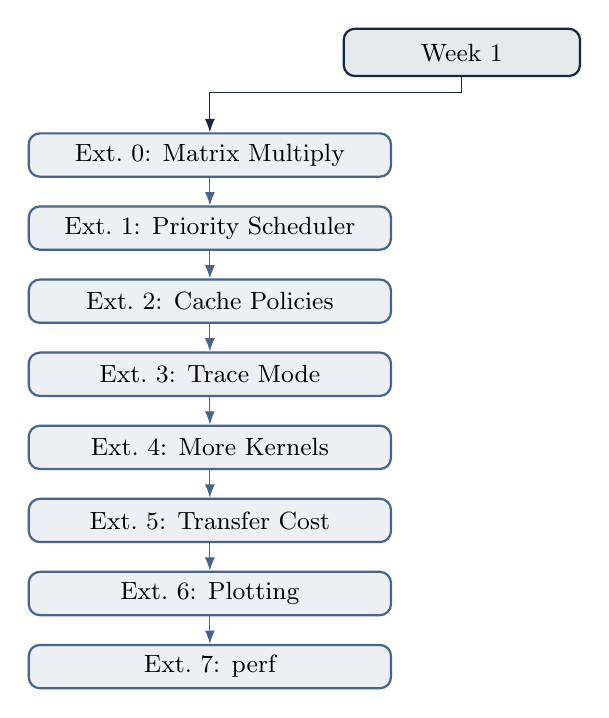
\begin{tikzpicture}[
  every node/.style={font=\small},
  box/.style={draw=steel, thick, rounded corners, fill=steel!10, minimum width=4.6cm, minimum height=0.55cm, align=center},
  wk/.style={draw=navy, thick, rounded corners, fill=navy!10, minimum width=3cm, minimum height=0.6cm, align=center},
  node distance=0.35cm
]
\node[wk] (wk1) {Week 1};
\node[box, below=0.7cm of wk1, xshift=-3.2cm] (e0) {Ext.\ 0: Matrix Multiply};
\node[box, below=of e0] (e1) {Ext.\ 1: Priority Scheduler};
\node[box, below=of e1] (e2) {Ext.\ 2: Cache Policies};
\node[box, below=of e2] (e3) {Ext.\ 3: Trace Mode};
\node[box, below=of e3] (e4) {Ext.\ 4: More Kernels};
\node[box, below=of e4] (e5) {Ext.\ 5: Transfer Cost};
\node[box, below=of e5] (e6) {Ext.\ 6: Plotting};
\node[box, below=of e6] (e7) {Ext.\ 7: perf};

\draw[-{Latex}, navy] (wk1.south) -- ++(0,-0.2) -| (e0.north);
\foreach \a/\b in {e0/e1, e1/e2, e2/e3, e3/e4, e4/e5, e5/e6, e6/e7}
  \draw[-{Latex}, steel] (\a) -- (\b);
\end{tikzpicture}
\end{center}

\begin{center}
\begin{tabularx}{\textwidth}{@{}p{2.4cm}X@{}}
\toprule
\textbf{Extension} & \textbf{Depends on} \\
\midrule
0 --- Matrix Multiply & Vector Add kernel + shared memory (Week~1); skipped
entirely if it already landed in Week~1 \\
1 --- Priority Scheduler & \texttt{WarpScheduler} interface (Day~3) \\
2 --- Cache Policies & \texttt{ReplacementPolicy} interface (Day~4) \\
3 --- Trace Mode & Scheduler + memory hierarchy functional
(Week~1 complete) \\
4 --- More Kernels & Kernel-launch plumbing (Week~1); Reduction additionally
depends on the barrier implementation \\
5 --- Transfer Cost & Kernel-launch infrastructure + performance-counter
reporting (Week~1) \\
6 --- Plotting & Any CSV output existing (true from Week~1 onward) \\
7 --- \texttt{perf} & A working, measurable simulator build (Week~1
complete) \\
\bottomrule
\end{tabularx}
\end{center}

Each extension only touches interfaces already built abstractly in Week~1
--- there is no risk of breaking Week~1's working core, and each
weekend's work is independently shippable.

% =========================================================
% RECOMMENDED LONG-TERM SEQUENCING
% =========================================================
\section{Recommended Long-Term Sequencing}

\begin{center}
\fbox{\begin{minipage}{0.85\textwidth}
\centering
This sequencing is \textbf{post-Week-1} --- it is not part of the
seven-day MVP.
\end{minipage}}
\end{center}

\begin{center}
\begin{tabularx}{\textwidth}{@{}p{2cm}X@{}}
\toprule
\textbf{Weekend} & \textbf{Work} \\
\midrule
+1 & Extension 0 (matrix multiply, only if it did not land in Week~1) \\
+2 & Extension 1 (priority scheduler) + Extension 2 (FIFO/Random cache
policies) \\
+3 & Extension 3 (debug/trace mode) \\
+4 & Extension 4 (additional benchmark kernels --- memcpy/streaming and
reduction are the highest-value pair if time is limited) \\
+5 & Extension 5 (transfer cost model) \\
+6 & Extension 6 (plotting) then Extension 7 (\texttt{perf}) only if time
remains \\
\bottomrule
\end{tabularx}
\end{center}

If Tiled Matrix Multiply landed during Week~1, Extension~0 is skipped
entirely and work begins at Extension~1.

% =========================================================
% TESTING STRATEGY
% =========================================================
\section{Testing Strategy}

\begin{longtable}{@{}p{3.2cm}p{11.3cm}@{}}
\toprule
\textbf{Component} & \textbf{Coverage} \\
\midrule
\endhead
Architecture & Hierarchy construction, warp formation, partial warps,
block formation, empty grid. \\
Instruction execution & Arithmetic correctness, register behavior,
load/store, branching, barrier instruction handling. \\
Scheduler & Round-Robin ordering, Greedy behavior, completion guarantees,
stall handling. \\
Cache & Hit, miss, eviction, associativity, LRU correctness, L1/L2
behavior. \\
Memory & Register file, shared memory, global memory, coalescing
classification. \\
Synchronization & Valid barrier completion, malformed/divergent barrier
detection, deadlock (hang) prevention. \\
Occupancy & Resource-constraint handling, resident block calculation,
active warp calculation. \\
\bottomrule
\end{longtable}

The final Week~1 target is approximately 30--50 meaningful tests
(Section~\ref{sec:day7}); the README reports the actual, measured \texttt{ctest}
count from the final run rather than this target figure.

% =========================================================
% MEASUREMENT INTEGRITY
% =========================================================
\section{Measurement Integrity}
\label{sec:measurement-integrity}

\begin{itemize}[leftmargin=1.2cm]
  \item Benchmark numbers must come from real simulator runs.
  \item No fabricated numbers, anywhere in the README or this roadmap's
  companion status report.
  \item No placeholder performance claims in the final README.
  \item CSV files contain actual measured values only.
  \item Benchmark configurations must be reproducible from the checked-in
  config files.
  \item This roadmap itself never implies that the illustrative numbers it
  contains (e.g.\ example cycle counts, example hit rates) are actual
  results --- every such figure in this document is drawn directly from
  the planning documents as an \textbf{illustrative example}, not a
  measurement.
\end{itemize}

% =========================================================
% CSV / EXPERIMENT DATA MODEL
% =========================================================
\section{CSV / Experiment Data Model}

A consistent schema keeps all four (and later, additional) experiments
comparable. Proposed fields:

\begin{center}
\begin{tabularx}{\textwidth}{@{}p{4cm}X@{}}
\toprule
\textbf{Field} & \textbf{Meaning} \\
\midrule
\texttt{experiment} & Experiment identifier (e.g.\ \texttt{scheduler\_comparison}) \\
\texttt{configuration} & Config file / label used for the run \\
\texttt{scheduler} & Scheduling policy, where applicable \\
\texttt{block\_size} & Threads per block, where applicable \\
\texttt{cache\_size} & Cache size, where applicable \\
\texttt{access\_pattern} & Contiguous / strided / random, where applicable \\
\texttt{cycles} & Total simulated cycles \\
\texttt{instructions\_retired} & Total instructions retired \\
\texttt{ipc} & Instructions per cycle \\
\texttt{stalls} & Stall count by reason \\
\texttt{cache\_hits} / \texttt{cache\_misses} & Cache statistics \\
\texttt{memory\_transactions} & Coalesced transaction count \\
\texttt{amat} & Average memory access time \\
\texttt{occupancy} & Computed occupancy \\
\texttt{throughput} & Kernel throughput metric \\
\bottomrule
\end{tabularx}
\end{center}

Only fields actually relevant to a given experiment need to be populated
--- for example, the coalescing experiment need not report
\texttt{occupancy}, and the block-size experiment need not report
\texttt{amat}. No experiment is forced to report every metric.

% =========================================================
% REPOSITORY STRUCTURE
% =========================================================
\section{Repository Structure}

\begin{lstlisting}
SIM-SM/
|-- CMakeLists.txt
|-- README.md
|-- configs/
|-- include/
|-- src/
|-- tests/
|-- results/
`-- scripts/
\end{lstlisting}

\begin{center}
\fbox{\begin{minipage}{0.85\textwidth}
\centering
The repository structure is intentionally small and modular.
\end{minipage}}
\end{center}

% =========================================================
% MAJOR INTERFACES
% =========================================================
\section{Major Interfaces}

\begin{lstlisting}
WarpScheduler
|-- RoundRobinScheduler
`-- GreedyScheduler
\end{lstlisting}

\begin{lstlisting}
Cache
|-- sets
|-- lines
|-- associativity
`-- ReplacementPolicy
\end{lstlisting}

\begin{lstlisting}
ReplacementPolicy
`-- LRUPolicy            (Week 1; FIFOPolicy / RandomPolicy in Extension 2)
\end{lstlisting}

\begin{lstlisting}
PerformanceCounter
|-- cycles
|-- instructions retired
|-- IPC
|-- stalls
|-- cache statistics
`-- memory transactions
\end{lstlisting}

Post-Week-1 extensions attach to these same three interfaces
(\texttt{WarpScheduler} gains \texttt{PriorityScheduler};
\texttt{ReplacementPolicy} gains \texttt{FIFOPolicy} and
\texttt{RandomPolicy} alongside Week~1's \texttt{LRUPolicy}; the
debug/trace mode attaches as a second observer of
\texttt{PerformanceCounter} events) rather than requiring new top-level
interfaces.

% =========================================================
% SIMPLIFICATIONS VS REAL GPU HARDWARE
% =========================================================
\section{Simplifications vs. Real GPU Hardware}
\label{sec:simplifications}

\begin{longtable}{@{}p{3cm}p{6cm}p{6cm}@{}}
\toprule
\textbf{Aspect} & \textbf{SIM-SM} & \textbf{Real GPU} \\
\midrule
\endhead
SM execution & Single-threaded C++ process simulating SM behavior
sequentially & Massively parallel hardware execution units \\
Warp scheduling & Two (later three) simplified policies: Round-Robin,
Greedy, (Priority) & Complex hardware schedulers with many additional
signals (e.g.\ dependency stalls, dual-issue, hardware-specific
heuristics) \\
SIMT & Lockstep execution of a tiny custom ISA & Real SIMT execution over
a full, hardware-specific instruction set \\
Divergence & One constrained branch pattern in Week~1 (no general
reconvergence stack) & General-purpose reconvergence hardware handling
arbitrary control flow \\
Memory & Modeled registers/shared/global memory with simplified timing &
Physical memory subsystems with real electrical and timing
characteristics \\
Cache & Configurable set/line/associativity model with LRU (later
FIFO/Random) & Hardware caches with proprietary, often adaptive
replacement policies \\
Synchronization & Simplified block-level barrier with explicit
malformed-case detection & Hardware synchronization primitives with
additional guarantees and failure modes \\
Timing & Abstract cycle counting via simulator logic & Real clock-driven
hardware timing \\
Instruction set & Minimal custom 9-opcode ISA & Full, proprietary,
hardware-specific instruction set (e.g.\ real PTX/SASS) \\
Occupancy & Computed from a simplified resource model & Computed from real
hardware resource limits and scheduling constraints \\
\bottomrule
\end{longtable}

SIM-SM does not claim fidelity to any of the real-GPU columns above; the
comparison exists specifically so that gap is explicit and undeniable, for
both the README and any interview discussion.

% =========================================================
% INTERVIEW TALKING POINTS
% =========================================================
\section{Interview-Defensible Technical Story}

\begin{description}[leftmargin=1cm, style=nextline]
  \item[Why build a GPU simulator?] To demonstrate systems-level
  understanding of parallel execution, scheduling, and memory hierarchy
  design in working code, without requiring access to real GPU hardware
  internals or driver-level tooling.
  \item[Why C++?] It is the language of real systems and performance-critical
  software, and matches the level of control needed to model registers,
  memory, and cycle-level counters directly.
  \item[Why model warps?] Warp-granularity execution is the core SIMT
  abstraction; modeling it directly is what makes scheduling and
  divergence experiments meaningful rather than abstract.
  \item[Why compare Round-Robin and Greedy?] It isolates scheduling policy
  as the single variable and produces a measured, explainable difference
  in cycles and IPC --- the clearest possible demonstration that
  scheduling policy matters.
  \item[Why model cache hierarchy?] Memory behavior dominates real GPU
  performance; modeling L1/L2 with configurable parameters makes cache
  effects measurable rather than assumed.
  \item[Why LRU?] It is the standard baseline replacement policy, and (per
  Extension~2) is deliberately shown to be non-universally-optimal with a
  measured counter-example, avoiding the trap of treating it as obviously
  correct.
  \item[Why memory coalescing?] It is one of the most consequential,
  most teachable GPU-specific memory-access effects, and is directly
  measurable as a transaction-count difference.
  \item[Why occupancy?] It ties resource constraints (registers, shared
  memory, threads/block) to actual scheduling outcomes, connecting
  architecture to measured throughput.
  \item[Why barrier synchronization?] Synchronization correctness is a
  first-class systems concern; detecting malformed/divergent barrier usage
  instead of allowing a silent hang is itself a real engineering
  requirement, not a cosmetic feature.
  \item[Why Vector Add?] It is the simplest kernel that still supports all
  four required experiments cleanly, keeping Week~1 feasible while still
  producing a complete, defensible set of measurements.
  \item[Why not implement CUDA/PTX?] That is real driver/runtime/ISA
  engineering with a completely different scope and risk profile; SIM-SM's
  goal is architectural and systems reasoning, not reproducing a
  proprietary instruction set or runtime.
  \item[What is simplified compared with a real GPU?] See
  Section~\ref{sec:simplifications} --- SM execution, scheduling, SIMT, divergence, memory,
  cache, synchronization, timing, instruction set, and occupancy are all
  simplified relative to real hardware, explicitly and by design.
  \item[What did you measure?] Whatever is actually in the checked-in CSV
  files at the time of the interview --- cycles, IPC, stalls, cache hit
  rate, memory transactions, and occupancy across the four Week~1
  experiments, plus any extension-specific measurements completed by that
  point.
  \item[What would you build next?] Whichever post-Week-1 extension is
  next in the roadmap at that time (Section~\ref{sec:post-week1}), in the stated priority
  order.
\end{description}

% =========================================================
% RESUME ALIGNMENT
% =========================================================
\section{Resume Alignment}

\textbf{Current framing} (usable now, while Week~1 is in progress --- these
describe the project as being actively built, not as already complete):

\begin{quote}
\itshape
Building a configurable GPU architecture simulator in C++, modeling SMs,
32-thread SIMT warps, and a multi-level memory hierarchy spanning
registers, shared memory, L1/L2 cache, and global memory.
\end{quote}

\begin{quote}
\itshape
Extending the simulator with pluggable Round-Robin and Greedy warp
scheduling atop an LRU-cached memory hierarchy, tracking execution
cycles, IPC, stalls, and cache hit rates across configurable workloads.
\end{quote}

\textbf{Completed-tense equivalents} (switch to these only once Week~1's
hierarchy, scheduling, memory/cache stack, and experiments are actually
built, compiled, run, and measured):

\begin{quote}
\itshape
Implemented a configurable GPU architecture simulator in C++ modeling
SM-level warp scheduling, SIMT execution with branch divergence, and a
multi-level memory hierarchy (registers/shared/L1/L2/global) with LRU
caching and memory coalescing.
\end{quote}

\begin{quote}
\itshape
Benchmarked round-robin vs.\ greedy warp scheduling, cache size, memory
access patterns, and block size/occupancy on a vector-add kernel,
measuring cycles, IPC, cache hit rate, memory transactions, and occupancy
across each experiment.
\end{quote}

If matrix multiply lands (either in Week~1 or as Extension~0), the second
bullet may say "vector-add and tiled matrix-multiply kernels" --- updated
only once it is actually built and measured.

\textbf{Updated bullets once Extensions 1, 2, 3, and 5 are complete}
(a realistic "solid v2"):

\begin{quote}
\itshape
Extended a C++ GPU architecture simulator with a third pluggable
warp-scheduling policy and two additional cache replacement policies, and
added a per-cycle debug trace mode for scheduler/memory state inspection.
\end{quote}

\begin{quote}
\itshape
Modeled host-device transfer cost separately from on-device execution
time, identifying and measuring the problem-size crossover point where
transfer overhead stops dominating total runtime.
\end{quote}

\begin{center}
\fbox{\begin{minipage}{0.85\textwidth}
\centering
Resume claims should only be updated once the corresponding implementation
actually exists, compiles, runs, and has been tested/measured. Every
resume bullet must be traceable to code that exists and ran.
\end{minipage}}
\end{center}

% =========================================================
% DEFINITION OF DONE
% =========================================================
\section{Definition of Done}

\subsection{Week 1 Done}

\begin{itemize}[leftmargin=1.2cm]
  \item[$\square$] Clean CMake build
  \item[$\square$] GoogleTest passes
  \item[$\square$] JSON configuration
  \item[$\square$] GPU/SM/Block/Warp/Thread hierarchy
  \item[$\square$] Toy ISA
  \item[$\square$] Instruction execution
  \item[$\square$] Round-Robin scheduler
  \item[$\square$] Greedy scheduler
  \item[$\square$] Performance counters
  \item[$\square$] Register file
  \item[$\square$] Shared memory
  \item[$\square$] Global memory
  \item[$\square$] L1 cache
  \item[$\square$] L2 cache
  \item[$\square$] LRU replacement
  \item[$\square$] AMAT calculation
  \item[$\square$] Memory coalescing
  \item[$\square$] Constrained divergence
  \item[$\square$] Barrier synchronization
  \item[$\square$] Barrier failure detection
  \item[$\square$] Occupancy calculation
  \item[$\square$] Vector Add kernel
  \item[$\square$] Four controlled experiments
  \item[$\square$] Real CSV results
  \item[$\square$] Tests (real, meaningful, honestly counted)
  \item[$\square$] README
  \item[$\square$] Fresh-clone verification
\end{itemize}

\subsection{Post-Week-1}

Each extension (0 through 7) is tracked with its own proof-of-done
criterion, as specified in Section~\ref{sec:post-week1} --- an extension is only marked done
once its specific proof-of-done artifact (a correctness check, a CSV, a
captured trace, an embedded plot, etc.) actually exists in the repository.

% =========================================================
% RISK REGISTER
% =========================================================
\section{Risk Register}

\begin{longtable}{@{}p{3.6cm}p{2cm}p{2cm}p{6cm}@{}}
\toprule
\textbf{Risk} & \textbf{Probability} & \textbf{Impact} & \textbf{Mitigation} \\
\midrule
\endhead
Divergence / reconvergence complexity spiraling & High & High & Support
only the single constrained branch pattern (\texttt{thread\_id \% 2 == 0});
explicitly forbid building a general reconvergence stack in Week~1. \\
Barrier semantics allowing a silent hang & Medium & High & Treat
divergent-barrier detection as a correctness requirement; malformed
barrier usage must be detected and reported, never silently hung. \\
Execution/memory integration debugging & Medium & Medium & Budget Day~4
time for integration, not just cache-logic implementation; use hand-traced
unit tests to isolate cache correctness from integration bugs. \\
Cache integration issues & Medium & Medium & Validate the cache in
isolation via hand-traced access sequences before wiring it into the
execution loop. \\
\bottomrule
\end{longtable}

% =========================================================
% PROJECT EVOLUTION
% =========================================================
\section{Project Evolution}

\begin{center}
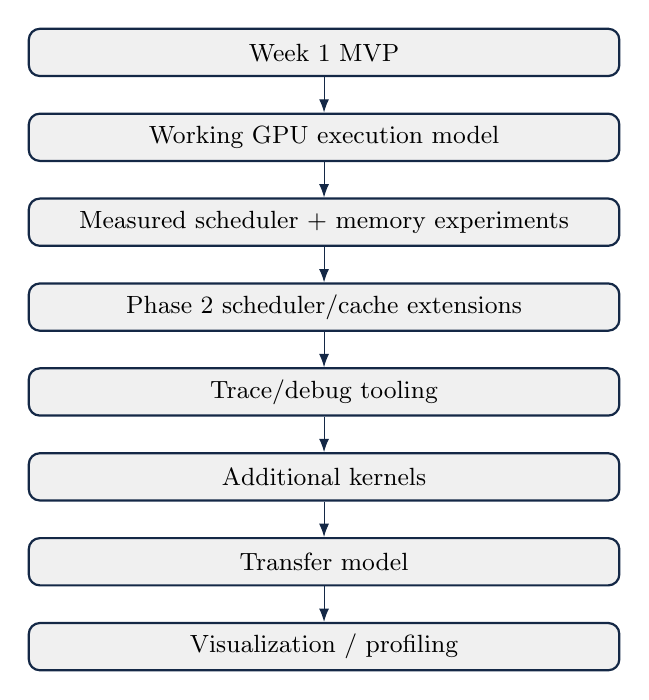
\begin{tikzpicture}[
  every node/.style={font=\small},
  stage/.style={draw=navy, thick, fill=lightgray, rounded corners, minimum width=7.5cm, minimum height=0.6cm, align=center},
  node distance=0.45cm
]
\node[stage] (a) {Week 1 MVP};
\node[stage, below=of a] (b) {Working GPU execution model};
\node[stage, below=of b] (c) {Measured scheduler + memory experiments};
\node[stage, below=of c] (d) {Phase 2 scheduler/cache extensions};
\node[stage, below=of d] (e) {Trace/debug tooling};
\node[stage, below=of e] (f) {Additional kernels};
\node[stage, below=of f] (g) {Transfer model};
\node[stage, below=of g] (h) {Visualization / profiling};

\foreach \x/\y in {a/b, b/c, c/d, d/e, e/f, f/g, g/h}
  \draw[-{Latex}, navy] (\x) -- (\y);
\end{tikzpicture}
\end{center}

\begin{center}
\fbox{\begin{minipage}{0.85\textwidth}
\centering
Build a small correct simulator first; extend only after the Week~1
interfaces are stable.
\end{minipage}}
\end{center}

\end{document}
